\documentclass[14pt,aspectratio=169,xcolor=dvipsnames]{beamer}
\usetheme{SimplePlus}
\usepackage{booktabs}
\usepackage{minted}

\title[short title]{Clase 4: Python, lenguaje e intérprete}
\subtitle{}
\author[NA Barnafi] {Nicolás Alejandro Barnafi Wittwer}
\institute[UC|CMM] 
{
    Pontificia Universidad Católica de Chile \\
    Centro de Modelamiento Matemático
}

\titlegraphic{
    \vspace{-1.8cm}
    \begin{flushright}
      
\includegraphics[height=2.5cm]{../images/logos/puc.png} 
    \end{flushright}
}

%\date{26/07/2024, Vancouver, WCCM}
\setbeamercovered{transparent}

\begin{document}
%%%%%%%%%%%%%%%%%%%%%%%%%%%%%%%%%%%%%%%%%%%%%%%%%%%%%%%
\begin{frame}
    \maketitle
\end{frame}
%%%%%%%%%%%%%%%%%%%%%%%%%%%%%%%%%%%%%%%%%%%%%%%%%%%%%%%
\begin{frame}\frametitle{Datos sobre Python}
    \begin{itemize}
        \item Lenguaje interpretado, orientado a objetos
        \item Creado en 1991 por Guido van Rossum
        \item Basado en C
        \item Librerías de IA: PyTorch, Keras, TensorFlow
        \item MUCHAS librerías científicas
        \item Ejecuta extensión \texttt{'.py'}
    \end{itemize}

\begin{block}{}
    \emph{[...] as a hobby project to keep himself busy during the Christmas holidays of 1989. }
\end{block}
\end{frame}
%%%%%%%%%%%%%%%%%%%%%%%%%%%%%%%%%%%%%%%%%%%%%%%%%%%%%%%
\begin{frame}\frametitle{Cómo usar Python}
    \begin{enumerate}
        \item<1-> Como programa
            \only<1>{
                \begin{flushright}
                    \texttt{nico@nico-pc:\~/Codes\$ python test.py}
                \end{flushright}
            }
        \item<2-> Como consola interactiva
            \only<2>{
                \begin{flushright}
                    \texttt{nico@nico-pc:\~/Codes\$ python} 
                    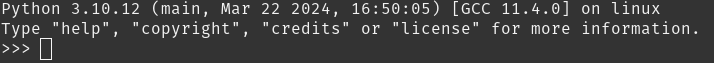
\includegraphics[width=0.9\textwidth]{../images/python-intepreter.png}
                \end{flushright}
            }
        \item<3-> \textbf{Jupyter/Collab/IDE (ayudantía)}
    \end{enumerate}

\vspace{1cm}
\idea{Veamos un poco la consola}
\end{frame}
%%%%%%%%%%%%%%%%%%%%%%%%%%%%%%%%%%%%%%%%%%%%%%%%%%%%%%%
\begin{frame}[t]\frametitle{Primeros códigos}
    \begin{itemize}
        \item Definición de variables (case sensitive)
            $$ > \underbrace{\texttt{a = 2}}_\text{Asignación \emph{siempre} de derecha a izquierda} $$
        \item Toda variable tiene un tipo 
            \begin{itemize}
                \item \texttt{> a = 2} : \hspace{0.3cm}\>\>\>\>\> 'a' es un 'int' (entero)
                \item \texttt{> a = 3.14}: \>\>\>\>\>'a' es un 'float' (punto flotante)
                \item \texttt{> a = "hola"}: 'a' es un 'string' (texto)
                \item \texttt{> a = True}: \>\>\> 'a' es un 'bool' (booleano)\footnote{esto tendrá sentido más adelante}
            \end{itemize}
        \item Se pueden dejar comentarios con \#
    \end{itemize}

\idea{Veamos en consola usando la función \texttt{type}}
\end{frame}
%%%%%%%%%%%%%%%%%%%%%%%%%%%%%%%%%%%%%%%%%%%%%%%%%%%%%%%
\begin{frame}\frametitle{Aritmética y propiedades algebráicas}
Cuál es el valor resultante de las siguientes operaciones? 

\vspace{1cm}
    \begin{itemize}
        \item \texttt{> a = 2+2}
        \item \texttt{> a = 2+2*2}
        \item \texttt{> a = 2/2*2}
        \item \texttt{> a = 2**2}   \textcolor{gray}{(elevado)}
        \item \texttt{> a = 'ho' + 'la'}
    \end{itemize}

\idea{Ojo: división entre enteros da un 'float'}

\end{frame}
%%%%%%%%%%%%%%%%%%%%%%%%%%%%%%%%%%%%%%%%%%%%%%%%%%%%%%%
\begin{frame}\frametitle{Nota sobre la división}
La división se entiende como aplicada exclusivamente al número precedente. Eso implica lo siguiente: 
    \begin{itemize}
        \item \texttt{2/2} es $\frac 2 2$
        \item \texttt{2/2*2} es $\left(\frac 2 2\right) \times 2$
        \item \texttt{2/2/2} es $\frac{\left(\frac 2 2\right)}{2}= \frac{2}{2\times 2}$
    \end{itemize}

\pause \idea{Es más fácil imaginar $a/b$ como $a b^{-1}$}
\end{frame}
%%%%%%%%%%%%%%%%%%%%%%%%%%%%%%%%%%%%%%%%%%%%%%%%%%%%%%%
\begin{frame}\frametitle{Álgebra booleana}
    Keywords importantes: 
    \begin{itemize}
        \item \texttt{and}, \texttt{or}, \texttt{not}
        \item \texttt{==}, \texttt{<=}, \texttt{>=}
    \end{itemize}

En términos de precedencia, \alertBlue{\texttt{and}} es un producto y \alertBlue{\texttt{or}} es una suma: 

$$ \texttt{a and b or c} = (\texttt{a and b}) \texttt{ or } c $$

Notar que el resultado es siempre otro booleano.
\end{frame}
%%%%%%%%%%%%%%%%%%%%%%%%%%%%%%%%%%%%%%%%%%%%%%%%%%%%%%%
\begin{frame}[fragile]\frametitle{Usando bools: if/then/else}

    \begin{minted}{python}
        d = 1 # Diámetro de figura
        if figuraEsCuadrado:
            area = d**2
        elif figuraEsCirculo:
            area = pi * (d/2)**2
        else # llego acá si no pasa otra
            print("Error")
    \end{minted}    
\end{frame}
%%%%%%%%%%%%%%%%%%%%%%%%%%%%%%%%%%%%%%%%%%%%%%%%%%%%%%%
\begin{frame}\frametitle{Recap}
    \begin{itemize}
        \item Python: lenguaje interpretado, orientado a objetos
        \item Usamos la consola interactiva de Python
        \item Tipos de variables: int, float, bool, string
        \item Operaciones entre variables, aritmética y álgebra
    \end{itemize}
\end{frame}
%%%%%%%%%%%%%%%%%%%%%%%%%%%%%%%%%%%%%%%%%%%%%%%%%%%%%%%
\begin{frame}
    \maketitle
\end{frame}
\end{document}
